
% !TEX encoding = UTF-8 Unicode 
% !TEX root = FieldGuide.tex

\Sec{Log-Normal Distribution} 
\label{sec:LogNormal}
\dist{Log-normal} (Galton, Galton-McAlister, anti-log-normal, Cobb-Douglas, log-Gaussian, logarithmic-normal, logarithmico-normal, $\Lambda$, Gibrat) distribution \cite{Galton1879, McAlister1879, Johnson1994}
 is  a three parameter, continuous, univariate, unimodal probability density with semi-infinite support. The functional form in the standard  parameterization is
 \begin{align}
 \label{LogNormal}
\opr{LogNormal}&(x\given a, \vartheta,\beta) 
 \\ \notag = & \frac{|\beta|}{\sqrt{2\pi \vartheta^2}} \left(\frac{x-a}{\vartheta}\right)^{-1} \exp\left\{-\frac{1}{2} \left(\beta \ln \frac{x-a}{\vartheta} \right)^2 \right\}  \checked
\\ \notag
& \text{ for } x,\ a,\ \vartheta,\ \beta \  \text{in } \Real,  	
 \\ \nonumber
 & \tfrac{x-a}{\vartheta}>0
\end{align}
The log-normal is so called because the log transform of the log-normal variate is a normal random variable. The distribution should, perhaps, be more accurately called the anti-log-normal distribution, but the nomenclature is now standard. 



\SSec{Special cases}
\phantomsection\addcontentsline{toc}{subsection}{~~~~~~~~~~~~Anchored log-normal} 
\phantomsection\addcontentsline{toc}{subsection}{~~~~~~~~~~~~Gibrat} 
The {\bf anchored log-normal} (two-parameter log-normal) distribution ($a=0$) arises from the multiplicative version of the central limit theorem: When the sum of independent random variables limits to normal, the product of those random variables limits to log-normal.
With $a=0$, $\vartheta=1$, $\sigma=1$  we obtain the  {\bf standard log-normal} (Gibrat) distribution~\cite{Gibrat1931}.


\SSec{Interrelations}
The log-normal forms a location-scale-power distribution family.
\begin{align*}
\opr{LogNormal}(a, \vartheta, \beta) &\sim a+ \vartheta  \oprr{StdLogNormal}{LogNormal}()^{1/\beta}
\checked
\end{align*}


The log-normal distribution is the anti-log transform of a normal random variable. 
\begin{align*}
\opr{LogNormal}(a, \vartheta, \beta) &\sim a+ \exp\Bigl(- \opr{Normal}(-\ln \vartheta,1/\beta)\Bigr) 
\checked
\end{align*}
Because of this close connection to the normal distribution, the log-normal is often parameterized with the mean and standard deviation of the corresponding normal distribution, $\mu=\ln \vartheta$, $\sigma=1/\beta$ rather than standard scale and power parameters. 


The log-normal distribution is a limiting form of the Unit gamma \eqref{UnitGamma} and Amoroso \eqref{Amoroso},  distributions (And therefore also of the generalized beta and generalized beta prime distributions) and limits to the normal distribution~\secref{sec:Limits}.
\[
\opr{Normal}(x\given \mu, \sigma)  =   \lim_{\beta\rightarrow\infty} \opr{LogNormal}(x\given \mu + \beta\sigma, -\beta\sigma, \beta) \checked
\notag
\]

A product of log-normal distributions (With zero location parameter) is again a log-normal distribution. This follows from the fact that the sum of normal distributions is normal.
\[
\prod_{i=1}^{n} \opr{LogNormal}_i(0, \vartheta_i, \beta_i) \sim 
\opr{LogNormal}_i(0, \prod_{i=1}^{n} \vartheta_i, (\sum_{i=0}^{n}\beta_i^{-2})^{-\half} ) 
\checked
\notag
\]


\begin{figure}[t]
\begin{center}
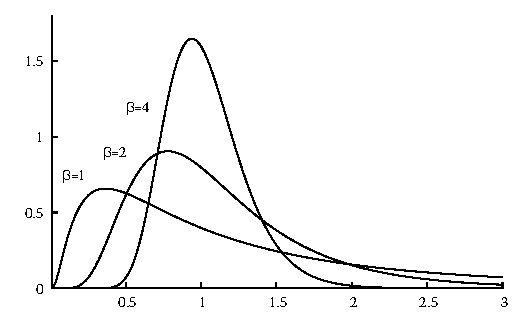
\includegraphics[width=\textwidth]{pdfLogNormal}
\end{center}
\caption[Log normal distributions]{Log normal distributions, $\opr{LogNormal}(x\given 0, 1, \beta)$}
\end{figure}







% !TEX encoding = UTF-8 Unicode 
% !TEX root = FieldGuide.tex

\begin{table*}[t!]
\caption[Log-normal distribution -- Properties]{Properties of the log-normal distribution}
 \begin{align*}
\text{\hyperref[PropertiesSec]{Properties}}  \quad& \\
\text{notation} \quad & \op{LogNormal}(x\given a, \vartheta,\beta ) \checked  	
\\
\text{PDF}\quad &   \frac{|\beta|}{\sqrt{2\pi \vartheta^2}} \left(\frac{x-a}{\vartheta}\right)^{-1} \exp\left\{-\frac{1}{2} \left( \beta \ln \frac{x-a}{\vartheta} \right)^2 \right\}	\checked					
\\
\text{CDF} \big/ \text{CCDF} \quad  &   \tfrac{1}{2} +  \tfrac{1}{2}\text{erf}\left( \sfrac{1}{\sqrt{2}} \beta \ln \frac{x-a}{\vartheta} \right) \checked
& \hspace{-2em} \vartheta >0 \ \big/ \ \vartheta <0
\\
\text{parameters}\quad &   a,\  \vartheta,\ \beta \text{ in } \Real		 \checked
\\
\text{support} \quad &   x \in [a, +\infty] \quad \vartheta>0 \checked
\\
& x \in [-\infty,a] \quad \vartheta<0 \checked
\\
\text{median} \quad  &  a+ \vartheta \checked
\\
\text{mode} \quad  & a+ \vartheta e^{-\beta^{-2}} \checked
\\
\text{mean} \quad  &  a + \vartheta e^{\tfrac{1}{2} \beta^{-2}} \checked
\\
\text{variance} \quad  & \vartheta^2 (e^{\beta^{-2}} -1) e^{\beta^{-2}} \checked
\\
\text{skew} \quad  &  ( e^{\beta^{-2}} +2) \sqrt{e^{\beta^{-2}} -1} \checked
\\
\text{kurtosis} \quad  &  e^{4\beta^{-2}} +2e^{3\beta^{-2}} +3e^{2\beta^{-2}} -6 \checked
\\
\text{entropy} \quad  & \tfrac{1}{2} + \tfrac{1}{2} \ln(2\pi\beta^{-2}) + \ln | \vartheta | \checked
\\
\text{MGF} \quad  &  \text{doesn't exist in general} \checked
\\
\text{CF} \quad  &  \text{no simple closed form expression} \checked
\end{align*}
\end{table*}


